\documentclass[a4paper, 12pt]{article}
\usepackage[utf8x]{inputenc}
\usepackage{cmap}
\usepackage[english, russian]{babel}
\usepackage{indentfirst}
\usepackage[left=20mm, top=20mm, right=20mm, bottom=20mm]{geometry}
\usepackage{tikz}
\usepackage{float}
\usepackage{amsmath, amsfonts, amssymb}
\usepackage{graphicx}
\usepackage{fancybox, fancyhdr}
\usepackage{hyperref}
\usepackage{listings}
\usepackage{caption}
\usepackage{subcaption}
\usepackage{xcolor}
\usepackage{paralist}
\pagestyle{fancy}
\fancyhf{}
\fancyhead[L]{Лабораторная работа №6}
\fancyhead[R]{Линейные системы автоматического управления}
\fancyfoot[C]{\thepage}
\graphicspath{{images/}}
\usetikzlibrary{patterns}
\definecolor{LightGray}{gray}{0.95}
\definecolor{LightGray2}{gray}{0.7}
\hypersetup{
    colorlinks=true,
    linkcolor=blue,
    filecolor=magenta,
    urlcolor=cyan,
    pdftitle={contents setup},
    pdfpagemode=FullScreen,
}
\setlength{\parskip}{1.5mm}
\setlength{\headheight}{15pt}
\setlength{\footskip}{15pt}
\allowdisplaybreaks

\begin{document}
    \begin{titlepage}

        \begin{center}
        
\includegraphics[width=0.3\textwidth]{itmo.png} % requires itmo.png in /images folder
        \vfill
        
        Федеральное государственное автономное образовательное учреждение высшего образования
        «Национальный Исследовательский Университет ИТМО»\\
        
        \vfill
        {\large\bf ЛАБОРАТОРНАЯ РАБОТА №6}\\
        {\large\bf ПРЕДМЕТ «ЛИНЕЙНЫЕ СИСТЕМЫ АВТОМАТИЧЕСКОГО УПРАВЛЕНИЯ»}\\
        {\large\bf ТЕМА «АНАЛИЗ ВЛИЯНИЯ НУЛЕЙ И ПОЛЮСОВ ПЕРЕДАТОЧНОЙ ФУНКЦИИ НА ДИНАМИЧЕСКИЕ СВОЙСТВА»}\\
        Вариант 4
        \vfill

        \begin{flushright}
            \begin{minipage}{.45\textwidth}
            {
                \hbox{Преподаватель: Золотаревич В. П.}
                \hbox{Студент: Румянцев А. А.}
                \hbox{Поток: ЛСАУ R22 бак 4.1.1}
                \hbox{}
                \hbox{Факультет: СУиР}
                \hbox{Группа: R3341}
            }
            \end{minipage}
        \end{flushright}
        
        \vfill
                
        Санкт-Петербург\\
        2024
        \end{center}
    \end{titlepage}
    
    \tableofcontents

    \newpage
    \section{Цель работы}
    Изучить связь характера переходной характеристики,
    динамических свойств системы с размещением на комплексной
    плоскости нулей и полюсов.


    \section{Задание 1}
    \subsection{Условие}
    По заданным значениям постоянных $$n=4,\ \ t_{\text{П}}=1.5,\ \ k=2.5,$$ определите
    параметры системы $$y^{(n)}+a_{n-1}y^{(n-1)}+...+a_1y^{(1)}+a_0y=bg$$
    с характеристическим полиномом Баттерворта и биномиальным полиномом.
    Для каждого случая рассчитайте корни характеристического полинома
    $$a(s)=s^n+a_{n-1}s^{n-1}+...+a_1s+a_0$$
    и оцените время переходного процесса по формуле $$t_{\text{П}}\approx\dfrac{1}{\eta}\ln{\dfrac{1}{0.05}}$$
    Составьте схему моделирования системы и постройте переходные характеристики,
    соответствующие двум типам распределения корней характеристического уравнения.


    \subsection{Выполнение}
    \textbf{Синтез системы с использованием полинома Баттерворта.}
    Полином Баттерворта в общем виде записывается как
    $$a(s)=\prod_{i=1}^{n}\left(s-\omega e^{j\left(\frac{\pi}{2}+\frac{2i-1}{2n}\pi\right)}\right)=s^n+\alpha_{n-1}\omega s^{n-1}+...+\alpha_1\omega^{n-1}s+\omega^n$$
    По графику нормированных переходных функций определим значение $t^*_{\text{П}}\Rightarrow t^*_{\text{П}}\approx6.8$
    \begin{figure}[H]
        \centering
        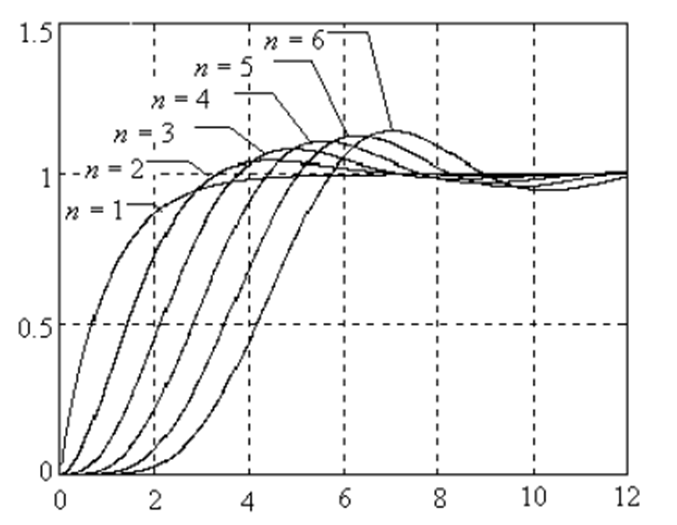
\includegraphics[scale=0.7]{norm_tf_bat.png}
        \captionsetup{skip=0pt}
        \caption{Нормированные переходные характеристики системы с характеристическим полиномом Баттерворта}
        \label{fig:norm_tf_bat}
    \end{figure}
    \noindent Найдем среднегеометрический корень $\omega_0$
    $$\omega_0=\sqrt[n]{|s_1s_2...s_n|}=\sqrt[n]{a_0}=\dfrac{t^*_{\text{П}}}{t_{\text{П}}}=\dfrac{6.8}{1.5}\approx4.53$$
    Коэффициенты полинома выражаются как
    $$a_j=\alpha_j\cdot\omega^{n-j}$$
    Для случая с $n=4$ (см. методическое пособие)
    $$
    \begin{matrix}
    \alpha_1=2.613\\
    \alpha_2=3.414\\
    \alpha_3=2.613
    \end{matrix}
    $$
    Полином Баттерворта для системы порядка $n=4$ имеет вид ($\alpha_3$ самый левый не единичный коэффициент, $\alpha_1$ самый правый)
    $$s^4+2.613\omega s^3+3.414\omega^2s^2+2.613\omega^3s+\omega^4$$
    Подставим найденный $\omega_0$, чтобы получить коэффициенты $a_j$. Полином Баттерворта для нашего случая будет иметь вид
    $$s^4+11.83689s^3+70.0583526s^2+242.903636s+421.1073368$$
    Найдем коэффициент $b$. Из полинома Баттерворта имеем коэффициент $$a_0=421.1073368,$$
    тогда $$b=k\cdot\omega^4=k\cdot a_0=2.5\cdot421.1073368=1052.768342$$
    Модель вход-выход системы будет иметь вид
    $$y^{(4)}+11.83689y^{(3)}+70.0583526y^{(2)}+242.903636y^{(1)}+421.1073368=1052.768342g$$
    Рассчитаем корни полинома по формуле
    $$s=\omega e^{j\left(\frac{\pi}{2}+\frac{2i-1}{2n}\pi\right)},\ i\in[1,2n]$$
    С учетом $\omega_0$ получим
    $$
    \begin{matrix}
    s_{1,4}=-1.7336\pm4.1852i\\
    s_{5,8}=\ \ \, 1.7336\mp4.1852i\\
    s_{2,3}=-4.1852\pm1.7336i\\
    s_{6,7}=\ \ \, 4.1852\mp1.7336i
    \end{matrix}
    $$
    Рассчитаем время переходного процесса. В качестве $\eta$ берется абсолютное значение вещественной части
    ближайшего к мнимой оси корня, то есть $$\eta=|\Re{\left(s_{1,4}\right)}|=1.7336$$
    $$t_{\text{П}}\approx\dfrac{1}{\eta}\ln{\dfrac{1}{0.05}}\approx\dfrac{3}{\eta}=\dfrac{3}{1.7336}\approx1.7305029995$$


    \textbf{Синтез системы с использованием полинома Ньютона.}
    Биномиальный полином в общем виде записывается как
    $$\alpha(s)=(s+\omega)^n=s^n+\alpha_{n-1}\omega s^{n-1}+...+\alpha_1\omega^{n-1}s+\omega^n$$
    По графику нормированных переходных функций определим значение $t^*_{\text{П}}\Rightarrow t^*_{\text{П}}\approx7.8$
    \begin{figure}[H]
        \centering
        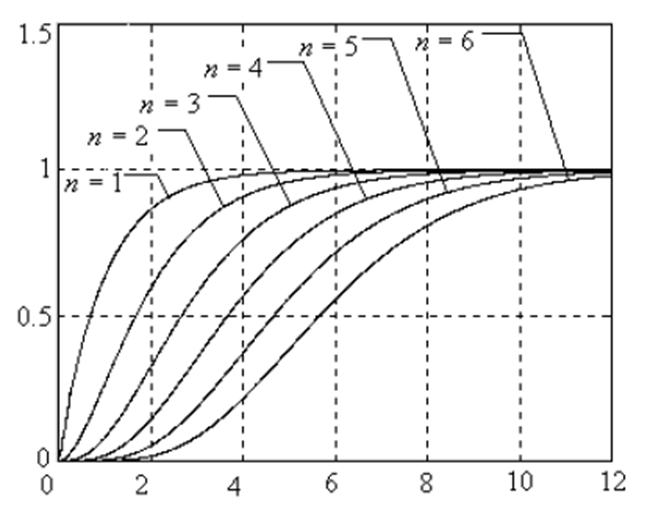
\includegraphics[scale=0.7]{norm_tf_newton.png}
        \captionsetup{skip=0pt}
        \caption{Нормированные переходные характеристики системы с биноминальным характеристическим полиномом}
        \label{fig:norm_tf_newton}
    \end{figure}
    \noindent Найдем среднегеометрический корень $\omega_0$
    $$\omega_0=\dfrac{t^*_{\text{П}}}{t_{\text{П}}}=\dfrac{7.8}{1.5}=5.2$$
    Коэффициенты полинома выражаются как
    $$a_j=\alpha_j\cdot\omega^{n-j}$$
    Для случая с $n=4$ (см. методическое пособие)
    $$
    \begin{matrix}
    \alpha_1=4\\
    \alpha_2=6\\
    \alpha_3=4
    \end{matrix}
    $$
    Биномиальный полином для системы порядка $n=4$ имеет вид ($\alpha_3$ самый левый не единичный коэффициент, $\alpha_1$ самый правый)
    $$s^4+4\omega s^3+6\omega^2s^2+4\omega^3s+\omega^4$$
    Подставим найденный $\omega_0$, чтобы получить коэффициенты $a_j$. Биномиальный полином для нашего случая будет иметь вид
    $$s^4+20.8s^3+162.24s^2+562.432s+731.1616$$
    Найдем коэффициент $b$. Из биномиального полинома имеем коэффициент $$a_0=731.1616,$$
    тогда $$b=k\cdot\omega^4=k\cdot a_0=2.5\cdot731.1616=1827.904$$
    Модель вход-выход системы будет иметь вид
    $$
    y^{(4)}+20.8y^{(3)}+162.24y^{(2)}+562.432y^{(1)}+731.1616=1827.904g
    $$
    При биномиальном распределении Ньютона $n$ комплексных чисел $s_i$ принимаются
    равными и вещественными, т.е. $s_i=-\omega$. Таким образом, $$s_i=-\omega_0=-5.2$$
    Рассчитаем время переходного процесса
    $$t_{\text{П}}\approx\dfrac{1}{\eta}\ln{\dfrac{1}{0.05}}\approx\dfrac{3}{\eta}=\dfrac{3}{5.2}\approx0.5769230769$$
    Схема моделирования двух полиномов представлена на рисунке \ref{fig:scheme1}.
    \begin{figure}[H]
        \centering
        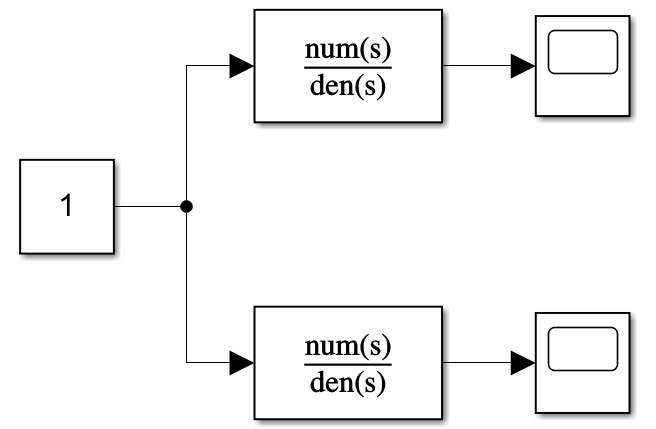
\includegraphics[scale=0.6]{scheme1.png}
        \captionsetup{skip=0pt}
        \caption{Схема эксперимента}
        \label{fig:scheme1}
    \end{figure}
    \noindent Параметры блоков ``Transfer Fcn'' в SIMULINK
    представлены на рисунке \ref{fig:windows1} под заголовком <<Приложения>>. Построим графики.
    \begin{figure}[H]
        \centering
        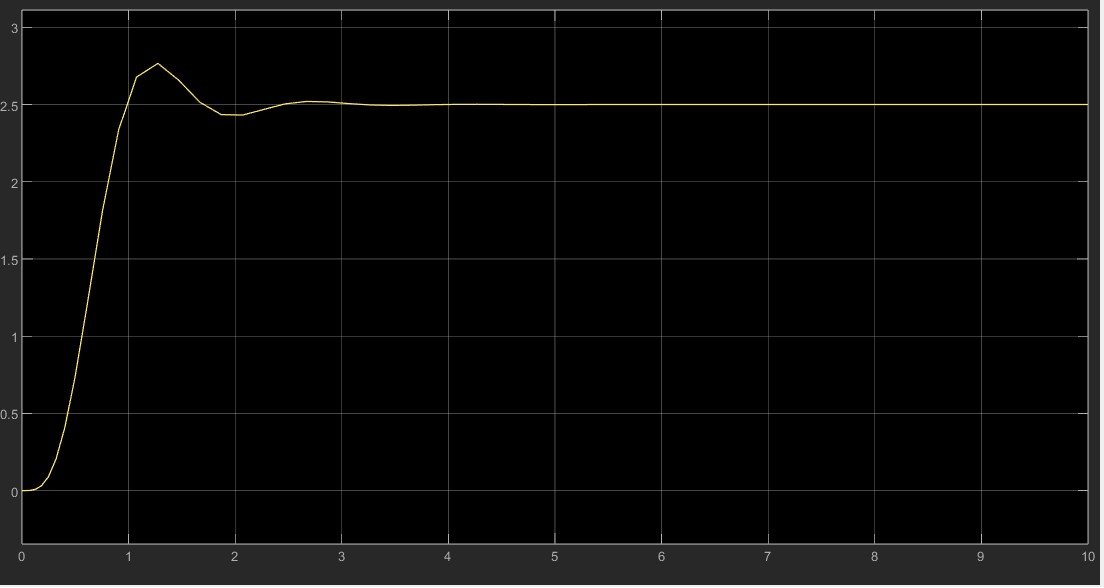
\includegraphics[scale=0.3]{task_1_baterwort.jpg}
        \captionsetup{skip=0pt}
        \caption{График переходной характеристики системы: полином Баттерворта}
        \label{fig:t1bat}
    \end{figure}
    \begin{figure}[H]
        \centering
        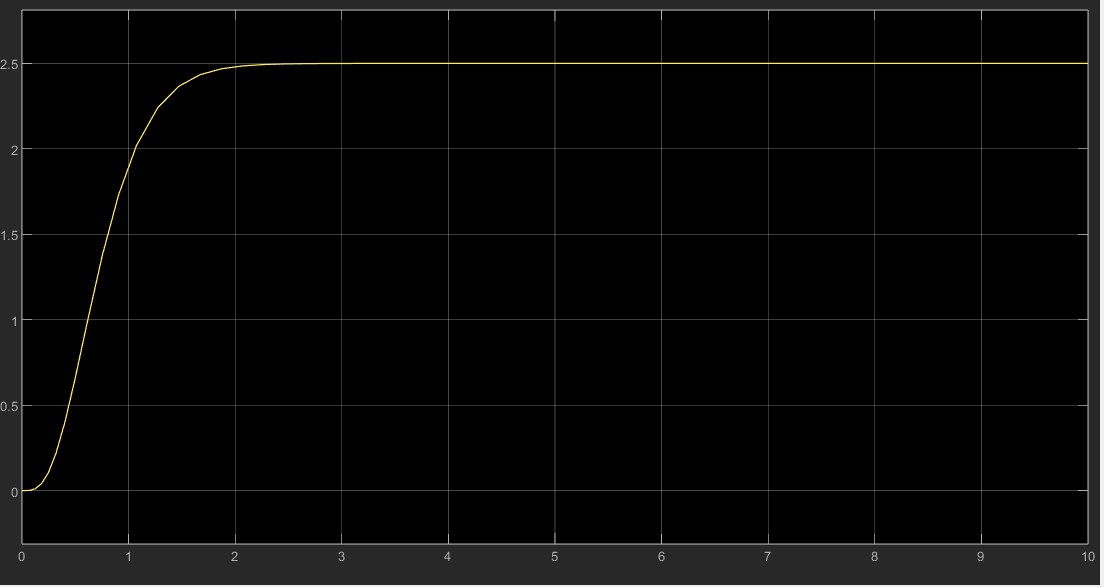
\includegraphics[scale=0.3]{task_1_newton.jpg}
        \captionsetup{skip=0pt}
        \caption{График переходной характеристики системы: полином Ньютона}
        \label{fig:t1newton}
    \end{figure}


    \section{Задание 2}
    \subsection{Условие}
    Для каждого набора параметров $$\text{A:}\ b_0=b,\ \ b_1=2.5$$
    $$\text{B:}\ b_0=b,\ \ b_1=0.5,\ \ b_2=0.25,\ \ b_3=1.25,\ \ b_4=2$$
    постройте переходные характеристики системы
    $$y^{(n)}+a_{n-1}y^{(n-1)}+...+a_1y^{(1)}+a_0y=b_mg^{(m)}+...+b_0g$$
    с коэффициентамиa $a_0,...,a_{n-1}$ и коэффициентом $b$,
    рассчитанными в первом задании для биномиального распределения
    корней характеристического уравнения.


    \subsection{Выполнение}
    \textbf{Пункт A.} Модель вход-выход системы будет иметь вид
    $$y^{(4)}+20.8y^{(3)}+162.24y^{(2)}+562.432y^{(1)}+731.1616=2.5g^{(1)}+1827.904g$$
    Схема моделирования представлена на рисунке \ref{fig:scheme2}.
    \begin{figure}[H]
        \centering
        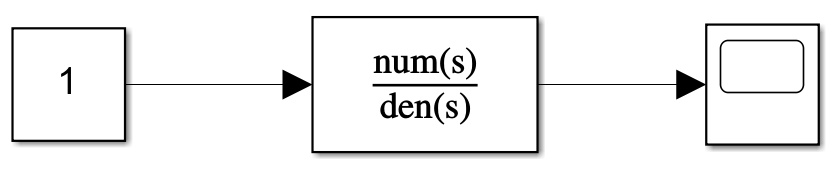
\includegraphics[scale=0.6]{scheme2.png}
        \captionsetup{skip=0pt}
        \caption{Схема эксперимента}
        \label{fig:scheme2}
    \end{figure}
    \noindent Параметры блока ``Transfer Fcn'' в SIMULINK
    представлены на рисунке \ref{fig:window2_A} под заголовком <<Приложения>>. Построим графики.
    \begin{figure}[H]
        \centering
        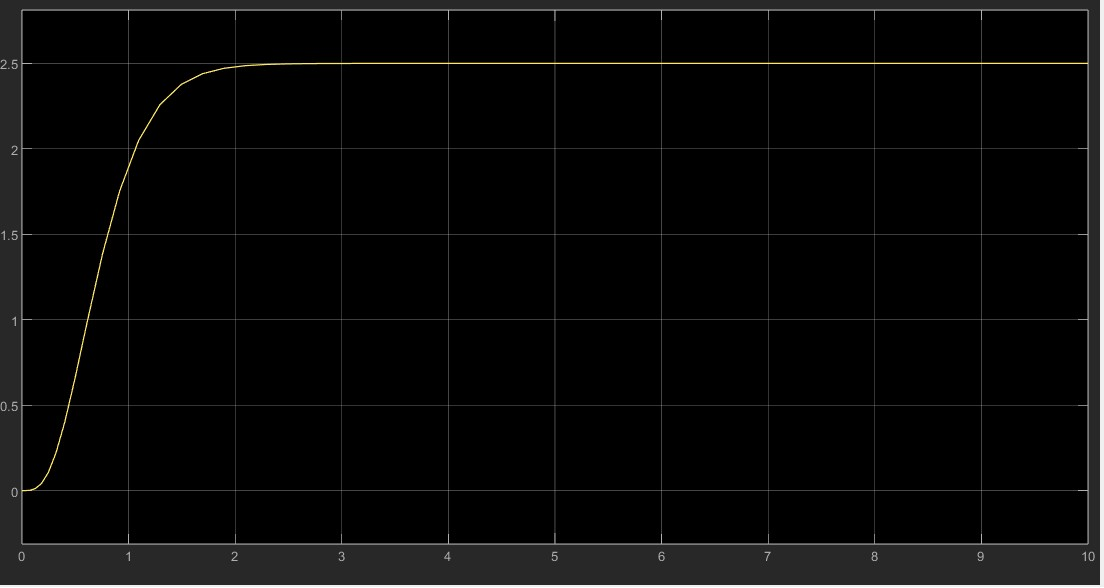
\includegraphics[scale=0.3]{task_2_A.jpg}
        \captionsetup{skip=0pt}
        \caption{График переходной характеристики системы}
        \label{fig:2A}
    \end{figure}


    \textbf{Пункт B.} Модель вход-выход системы будет иметь вид
    $$y^{(4)}+20.8y^{(3)}+162.24y^{(2)}+562.432y^{(1)}+731.1616=2g^{(4)}+1.25g^{(3)}+0.25g^{(2)}+0.5g^{(1)}+1827.904g$$
    Схема моделирования аналогична пункту A и представлена на рисунке \ref{fig:scheme2}.
    Параметры блока ``Transfer Fcn'' в SIMULINK
    представлены на рисунке \ref{fig:window2_B} под заголовком <<Приложения>>. Построим графики.
    \begin{figure}[H]
        \centering
        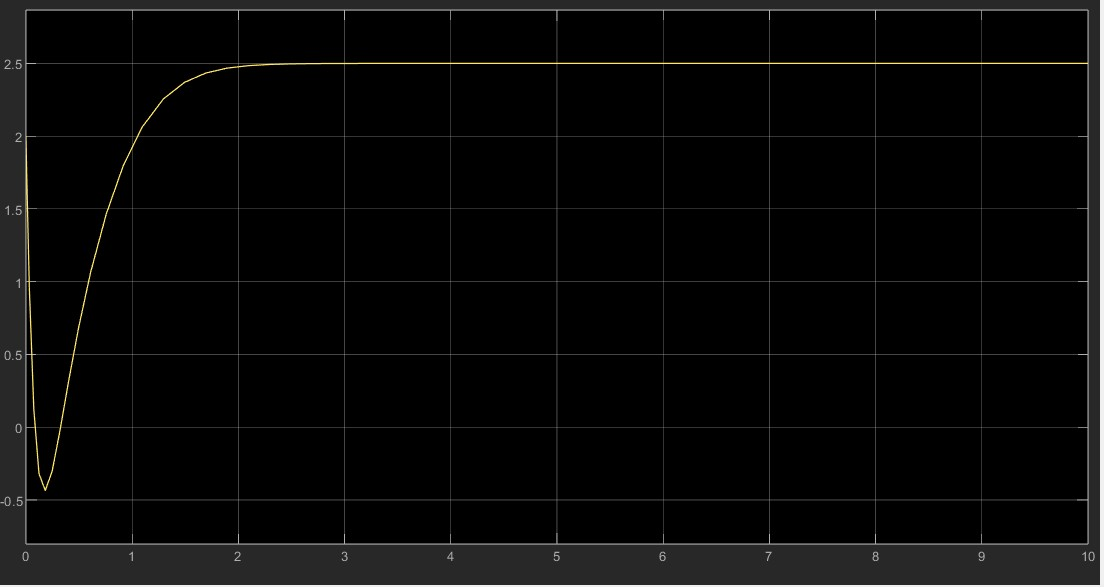
\includegraphics[scale=0.3]{task_2_B.jpg}
        \captionsetup{skip=0pt}
        \caption{График переходной характеристики системы}
        \label{fig:2B}
    \end{figure}


    \section{Задание 3}
    \subsection{Условие}
    Для набора параметров $$b_0=2.25,\ \ b_1=0,\ \ b_2=2$$ и внешнего воздействия
    $$g(t)=\sin{\left(1.5t\right)}$$ постройте реакцию системы
    $$y^{(n)}+a_{n-1}y^{(n-1)}+...+a_1y^{(1)}+a_0y=b_mg^{(m)}+...+b_0g$$ с нулевыми начальными
    условиями и коэффициентами $a_0,...,a_{n-1}$, рассчитанными
    в первом задании для биномиального распределения корней характеристического уравнения.
    На экран монитора выводить графики $y(t),g(t)$.


    \subsection{Выполнение}
    Модель вход-выход системы будет иметь вид
    $$y^{(4)}+20.8y^{(3)}+162.24y^{(2)}+562.432y^{(1)}+731.1616=2g^{(2)}+2.25$$
    Схема моделирования представлена на рисунке \ref{fig:scheme3}.
    \begin{figure}[H]
        \centering
        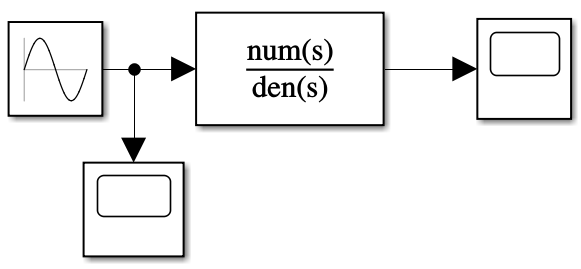
\includegraphics[scale=0.8]{scheme3.png}
        \captionsetup{skip=0pt}
        \caption{Схема эксперимента}
        \label{fig:scheme3}
    \end{figure}
    \noindent Параметры блока ``Transfer Fcn'' в SIMULINK
    представлены на рисунке \ref{fig:windows3} под заголовком <<Приложения>>. Построим графики.
    \begin{figure}[H]
        \centering
        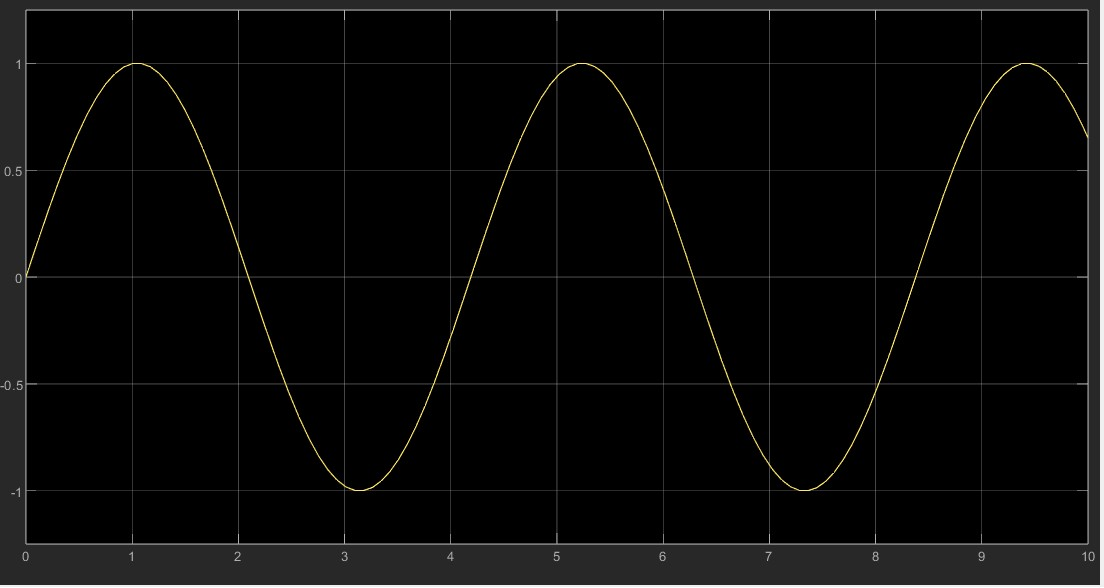
\includegraphics[scale=0.3]{task_3_g.jpg}
        \captionsetup{skip=0pt}
        \caption{График входного воздействия $g(t)$}
        \label{fig:gt2}
    \end{figure}
    \begin{figure}[H]
        \centering
        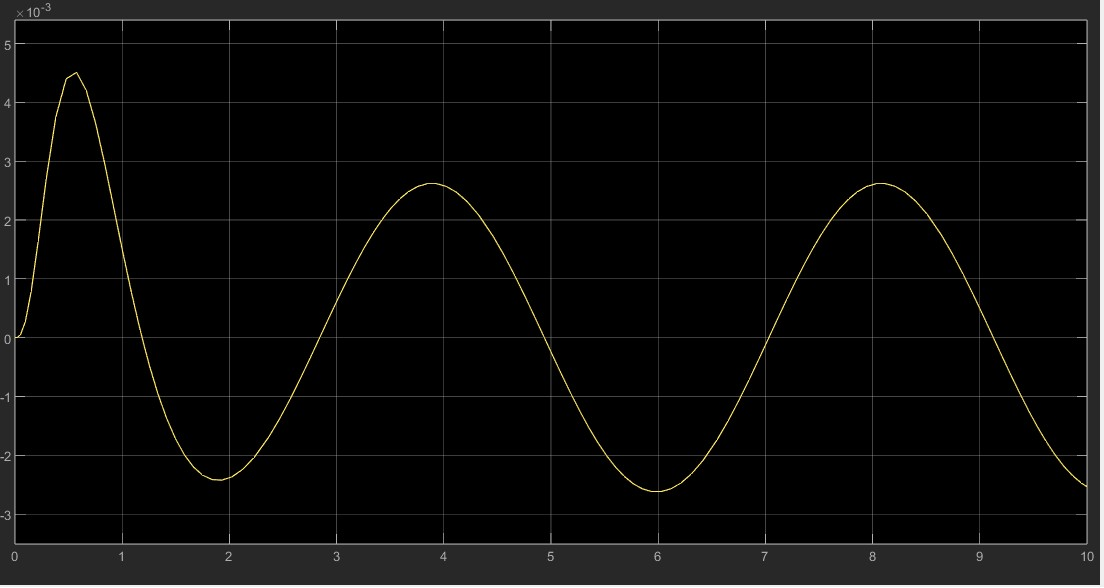
\includegraphics[scale=0.3]{task_3_y.jpg}
        \captionsetup{skip=0pt}
        \caption{График реакции системы $y(t)$}
        \label{fig:yt2}
    \end{figure}


    \section{Вывод}
    Я изучил связь характера переходной характеристики,
    динамических свойств системы с размещением на комплексной
    плоскости нулей и полюсов.


    На основе заданных параметров качества системы возможно выполнить её синтез,
    применяя стандартные переходные функции.
    Динамические характеристики системы находятся в прямой зависимости
    от полюсов и нулей её передаточной функции.


    \section{Приложения}
    \begin{figure}[H]
        \centering
        \begin{subfigure}{0.3\textwidth}
            \centering
            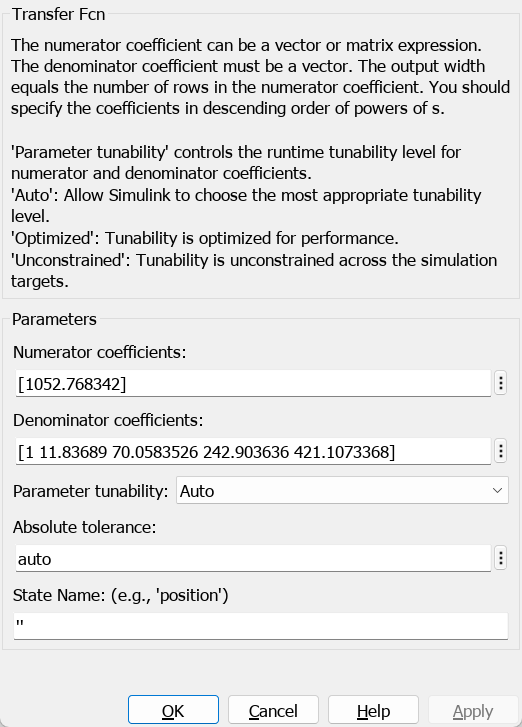
\includegraphics[width=\linewidth]{task1_baterwort_window.png}
            \caption{Параметры SIMULINK для полинома Баттерворта}
            \label{fig:t1bw}
        \end{subfigure}
        \begin{subfigure}{0.3\textwidth}
            \centering
            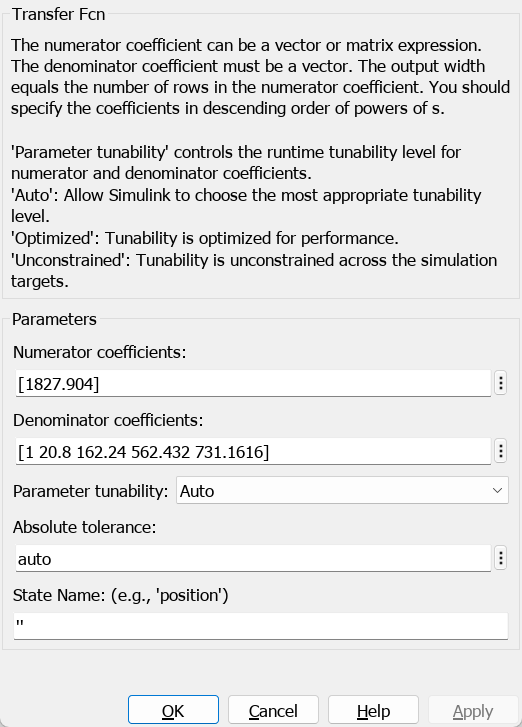
\includegraphics[width=\linewidth]{task1_newton_window.png}
            \caption{Параметры SIMULINK для полинома Ньютона}
            \label{fig:t1nw}
        \end{subfigure}
        \caption{Параметры SIMULINK для ``Transfer Fcn'' для задания 1}
        \label{fig:windows1}
    \end{figure}


    \begin{figure}[H]
        \centering
        \begin{subfigure}{0.3\textwidth}
            \centering
            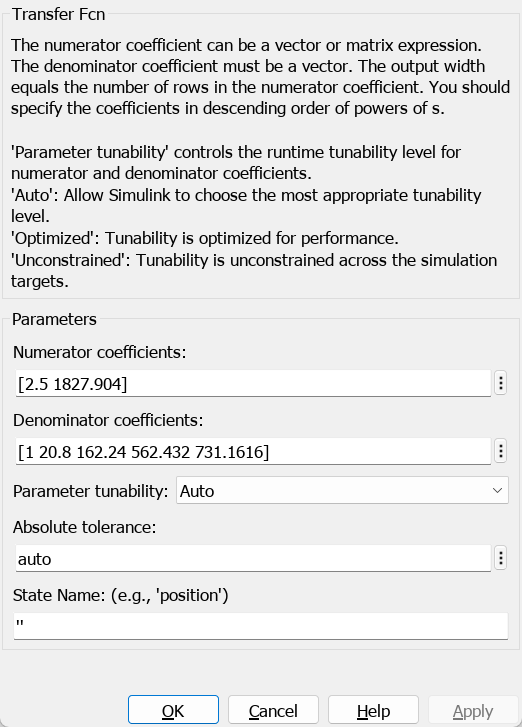
\includegraphics[width=\linewidth]{scheme2_window_A.png}
            \caption{Параметры SIMULINK переходной хар-ки системы A}
            \label{fig:window2_A}
        \end{subfigure}
        \begin{subfigure}{0.3\textwidth}
            \centering
            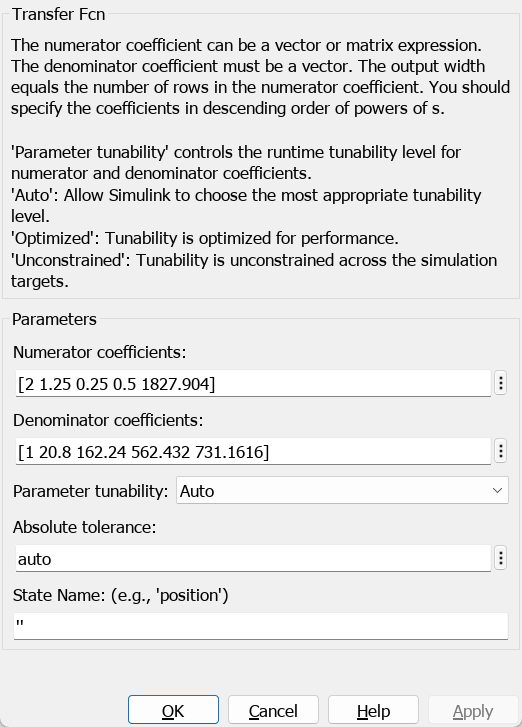
\includegraphics[width=\linewidth]{scheme2_window_B.png}
            \caption{Параметры SIMULINK переходной характеристики системы B}
            \label{fig:window2_B}
        \end{subfigure}
        \caption{Параметры SIMULINK для ``Transfer Fcn'' для задания 2}
        \label{fig:windows2}
    \end{figure}


    \begin{figure}[H]
        \centering
        \begin{subfigure}{0.3\textwidth}
            \centering
            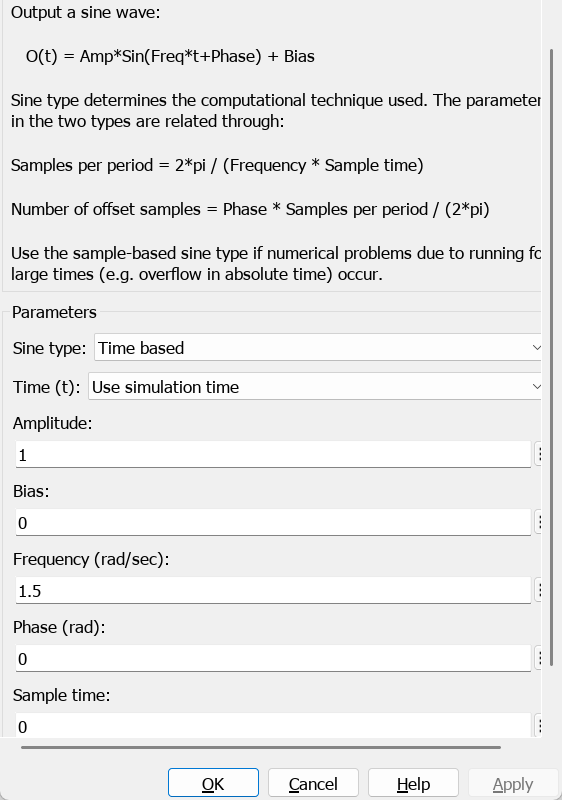
\includegraphics[width=\linewidth]{scheme3_window_sine.png}
            \caption{Параметры SIMULINK для входного сигнала $g(t)$}
            \label{fig:gt}
        \end{subfigure}
        \begin{subfigure}{0.3\textwidth}
            \centering
            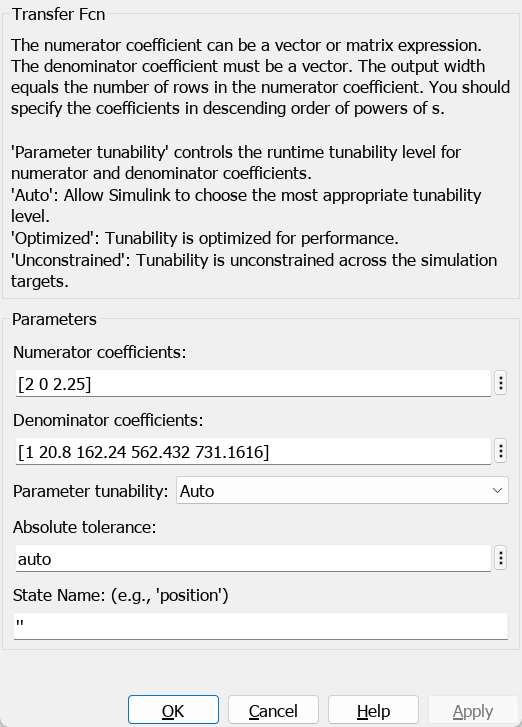
\includegraphics[width=\linewidth]{scheme3_window_tf.png}
            \caption{Параметры SIMULINK для реакции системы $y(t)$}
            \label{fig:yt}
        \end{subfigure}
        \caption{Параметры SIMULINK для ``Transfer Fcn'' для задания 3}
        \label{fig:windows3}
    \end{figure}
\end{document}